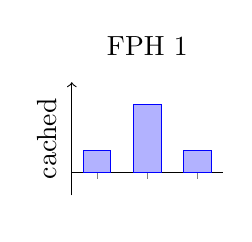
\begin{tikzpicture}
\begin{axis}[ybar, bar width={10pt}, title={FPH 1}, width={3.5cm}, ymin={-1}, ymax={4}, axis x line={middle}, axis y line={left}, xmin={0.5}, xmax={3.5}, xtick={1,2,3}, xticklabels={}, xticklabel shift={2mm}, y axis line style={{->}}, x axis line style={{-}}, ytick={\empty}, ylabel={cached}, ylabel style={yshift={0pt}}, yticklabels={f$_2$,f$_1$}, yticklabel={{\scriptsize
                                   \ifdim\tick pt < 0pt
                                   \pgfmathparse{-1*\tick}
                                   \pgfmathprintnumber{\pgfmathresult}
                                   \else
                                   \pgfmathprintnumber{\tick}
                                   \fi}}]
    \addplot
        coordinates {
            (1,1)
            (2,3)
            (3,1)
            (1,0)
            (2,0)
            (3,0)
        }
        ;
\end{axis}
\end{tikzpicture}
